% Created 2024-07-29 Mon 18:12
% Intended LaTeX compiler: pdflatex
\documentclass[letterpaper, 12pt]{article}
\usepackage[utf8]{inputenc}
\usepackage[T1]{fontenc}
\usepackage{graphicx}
\usepackage{longtable}
\usepackage{wrapfig}
\usepackage{rotating}
\usepackage[normalem]{ulem}
\usepackage{amsmath}
\usepackage{amssymb}
\usepackage{capt-of}
\usepackage{hyperref}
\usepackage{minted}
\usepackage{xcolor}
\usepackage{hyperref}
\usepackage{tocloft}
\usepackage{minted}
\usemintedstyle{manni}
\usepackage{pdfpages}
\usepackage{fancyhdr}
\usepackage{graphicx}
\usepackage[top=1.4in, left=0.5in, right=0.5in, bottom=0.8in]{geometry}
\usepackage[T1]{fontenc}
\usepackage{helvet}
\pagestyle{fancy}
\renewcommand{\headrulewidth}{0pt}
\renewcommand{\footrulewidth}{0pt}
\setlength{\parindent}{0em}
\setlength{\parskip}{1em}
\usepackage{hyperref}
\usepackage {color}
\usepackage {tabularray}
\usepackage{xcolor}
\hypersetup{
colorlinks=true,
linkcolor=blue,
filecolor=magenta,
urlcolor=cyan,
citecolor=green,
pdfborder={0 0 0}
}
\usepackage[most]{tcolorbox}
\author{Hilduara Abreu}
\date{\today}
\title{School Uniform Policy\\\medskip
\large Policy regarding the use of uniforms by students}
\hypersetup{
 pdfauthor={Hilduara Abreu},
 pdftitle={School Uniform Policy},
 pdfkeywords={},
 pdfsubject={},
 pdfcreator={Emacs 29.4 (Org mode 9.6.15)}, 
 pdflang={English}}
\begin{document}

\fancyfoot[C]{\setlength{\unitlength}{1in}\begin{picture}(5,0)\put(-1.8,-0.5){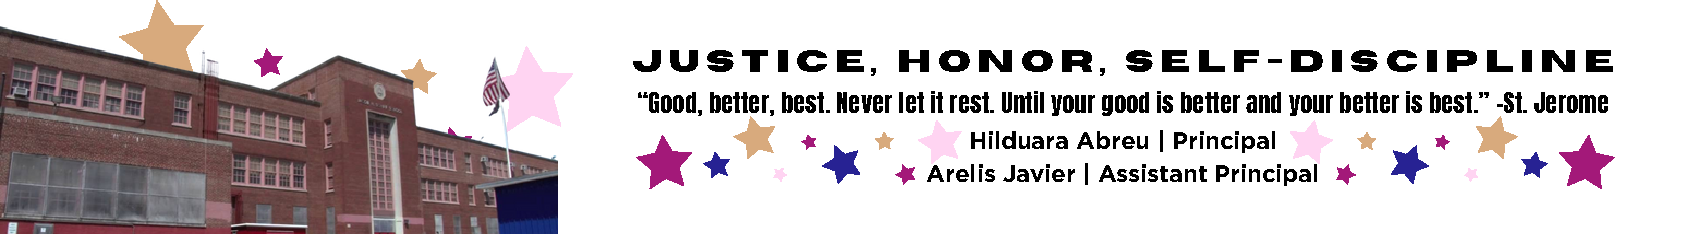
\includegraphics[width=8.8in,height=1.3in]{logo-1}}\end{picture}}
\fancyhead[C]{\setlength{\unitlength}{1in}\begin{picture}(5,0)\put(-1.9,-0.5){
\includegraphics[width=8.9in,height=1.3in]{logo-2}}\end{picture}}
\fancyhead[R]{\thepage}
\pagenumbering{gobble}

\begin{document}
\vspace*{-0.2in}
\tcbuselibrary{}
\newtcolorbox{bluebox}[1][]{
  colback=blue!5!white,
  colframe=blue!75!black,
  fonttitle=\bfseries,
  coltitle=black,
  enhanced,
  attach boxed title to top center={yshift=-2mm},
  title=#1,
  boxed title style={colback=blue!50!white}
}
\newtcolorbox{greenbox}[1][]{
  colback=green!5!white,
  colframe=green!75!black,
  fonttitle=\bfseries,
  coltitle=black,
  enhanced,
  attach boxed title to top center={yshift=-2mm},
  title=#1,
  boxed title style={colback=green!50!white}
}
\newtcolorbox{redbox}[1][]{
  colback=red!5!white,
  colframe=red!75!black,
  fonttitle=\bfseries,
  coltitle=black,
  enhanced,
  attach boxed title to top center={yshift=-2mm},
  title=#1,
  boxed title style={colback=red!50!white}
}

\section*{School Uniform Policy}
\label{sec:org9f06f41}
\begin{enumerate}
\item \hyperref[sec:org35f73c4]{English Version}
\item \hyperref[sec:org1d174bf]{Versión en Español}
\end{enumerate}
\pagebreak
\vspace*{-0.8cm}

\section*{English Version}
\label{sec:org35f73c4}
\textbf{\textbf{Uniform Details}}

\begin{enumerate}
\item \textbf{Burgundy Shirt}: All students are required to wear a burgundy-colored shirt as the upper part of their uniform.
\item \textbf{Navy Pants}: Navy blue pants or trousers are to be worn as the lower part of the uniform.
\end{enumerate}

The uniform policy will be enforced during school hours and at all school-related events and activities, such as field trips and special assemblies.

\textbf{\textbf{Benefits of the Uniform Policy}}

Uniforms serve as a unifying element within our school community and offer several significant advantages:

\begin{enumerate}
\item \textbf{Promoting Equality}: Uniforms eliminate socioeconomic disparities among students, ensuring that everyone is dressed the same way, regardless of their family’s financial circumstances.
\item \textbf{Enhancing Focus}: Wearing uniforms reduces distractions related to fashion and peer pressure, allowing students to concentrate on their studies and personal growth.
\item \textbf{Fostering School Pride}: A uniform instills a sense of pride and belonging among students, helping them identify with and appreciate their school community.
\item \textbf{Improving Safety}: Uniforms make it easier to identify intruders on school premises, enhancing overall security.
\item \textbf{Preparing for Future Success}: Encouraging a dress code similar to professional attire helps prepare students for future careers where a professional appearance is important.
\end{enumerate}

\textbf{\textbf{Dress Down Days}}

We understand that personal expression is important, and therefore, "Dress Down Days" will be occasionally scheduled throughout the school year, allowing students to express their individuality through clothing choices. We kindly request your cooperation and support in ensuring that your child arrives at school dressed in accordance with our uniform policy. We believe that this will contribute to a more positive and productive learning environment for all students.
\pagebreak
\vspace*{-0.5cm}

\textbf{\textbf{Contact Information}}

Should you have any questions or concerns regarding the uniform policy, please feel free to reach out to our Parent Coordinator, Ms. Angela Rijo, via the following channels:
\begin{itemize}
\item Website: \url{https://www.ps192.org/angela}
\item Whatsapp Group
\item ClassDojo
\item Phone: (212) 775-9560
\item In person during office hours: 9:00 AM - 3:00 PM
\end{itemize}

We are here to assist and support you.

\textbf{\textbf{Closing}}

Thank you for your partnership in nurturing a strong and vibrant learning community at P.S. 192. We look forward to a successful and enriching academic year ahead.

With Justice, Honor, and Self-Discipline,


\includegraphics[width=0.2\textwidth]{hil_signature}

\textbf{Hilduara Abreu, Principal}

\textbf{The School of Joyful Learning!}

\href{https://www.ps192.org}{www.ps192.org}

\pagebreak
\vspace*{-1cm}

\section*{Versión en Español}
\label{sec:org1d174bf}
\textbf{\textbf{Detalles del Uniforme}}

\begin{enumerate}
\item \textbf{Camisa Color Vino}: Se requiere que todos los estudiantes usen una camisa de color borgoña como la parte superior de su uniforme.
\item \textbf{Pantalones Azul Marino}: Pantalones o pantalones de color azul marino deben ser usados como la parte inferior del uniforme.
\end{enumerate}

La política de uniformes se aplicará durante el horario escolar y en todos los eventos y actividades relacionadas con la escuela, como excursiones y asambleas especiales.

\textbf{\textbf{Beneficios de la Política de Uniformes}}

Los uniformes sirven como un elemento unificador dentro de nuestra comunidad escolar y ofrecen varias ventajas significativas:

\begin{enumerate}
\item \textbf{Promoción de la Igualdad}: Los uniformes eliminan las disparidades socioeconómicas entre los estudiantes, asegurando que todos se vistan de la misma manera, independientemente de las circunstancias financieras de sus familias.
\item \textbf{Mejorando la Concentración}: Usar uniformes reduce las distracciones relacionadas con la moda y la presión de grupo, lo que permite a los estudiantes concentrarse en sus estudios y crecimiento personal.
\item \textbf{Fomento del Orgullo Escolar}: Un uniforme infunde un sentido de orgullo y pertenencia entre los estudiantes, ayudándolos a identificarse y apreciar su comunidad escolar.
\item \textbf{Mejora de la Seguridad}: Los uniformes hacen que sea más fácil identificar intrusos en las instalaciones escolares, mejorando la seguridad general.
\item \textbf{Preparación para el Éxito Futuro}: Fomentar un código de vestimenta similar a la vestimenta profesional ayuda a preparar a los estudiantes para futuras carreras donde una apariencia profesional es importante.
\end{enumerate}

\textbf{\textbf{Días de Ropa Libre}}
\pagebreak
\vspace*{-0.5cm}

Entendemos que la expresión personal es importante, y por lo tanto, los "Días de Ropa Libre" se programarán ocasionalmente a lo largo del año escolar, permitiendo a los estudiantes expresar su individualidad a través de sus elecciones de vestimenta. Solicitamos amablemente su cooperación y apoyo para asegurarse de que su hijo llegue a la escuela vestido de acuerdo con nuestra política de uniformes. Creemos que esto contribuirá a un ambiente de aprendizaje más positivo y productivo para todos los estudiantes.

\textbf{\textbf{Información de Contacto}}

Si tiene alguna pregunta o inquietud con respecto a la política de uniformes, no dude en ponerse en contacto con nuestra Coordinadora de Padres, Sra. Angela Rijo, a través de los siguientes canales:
\begin{itemize}
\item Sitio web: \url{https://www.ps192.org/angela}
\item Grupo de Whatsapp
\item ClassDojo
\item Teléfono: (212) 775-9560
\item En persona durante el horario de oficina: 9:00 AM - 3:00 PM
\end{itemize}

Estamos aquí para ayudar y apoyarlos.

\textbf{\textbf{Conclusión}}

Gracias por su colaboración en el fomento de una comunidad de aprendizaje fuerte y vibrante en P.S. 192. Esperamos un año académico exitoso y enriquecedor.

Con Justicia, Honor y Autodisciplina,


\includegraphics[width=0.2\textwidth]{hil_signature}

\textbf{Hilduara Abreu, Directora}

\textbf{¡La escuela del Aprendizaje Alegre!}

\href{https://www.ps192.org}{www.ps192.org}
\end{document}
